\section{Complexity}
\label{sect:complexity}
 
This section is dedicated to proving the NP-Completeness of the problem.

  \begin{theorem}
  \label{theo:complexity}
  The decision version of (MMC) is NP-Complete.
  \end{theorem}
  \begin{proof}
 

    Lets $M$ be an instance of MMC. Given an integer $K$, a subset $I$ of $\llbracket 1; p-1 \rrbracket$ and a subset $J$ of $\llbracket 1; q-1 \rrbracket$, one can compute in polynomial time the matrix $C(M,I,J)$ and checks if $d(C(M,I,J)) \geq K$. This proves the problem belongs to NP.

    In order to prove the NP-Hardness, we describe a polynomial reduction from the Maximum Clique problem. Lets $G(V,E)$ be an instance of the Maximum Clique problem, we build an instance $M$ of MMC with $p = q = (4|V| + 6)$. We arbitrarily number the nodes of $G$ : $V = \{v_1, v_2, \dots v_n\}$.

    Let $l_i$ and$c_i$ be respectively the $6+4(i-1)+1$-th line and the $6+4(i-1)+1$-th column. We associate the lines $l_i$ to $l_i+3$ and the columns $c_i$ to $c_i + 3$ to $v_i$. The key idea of the reduction is that each node $v$ is associated with two 1. If we chose the node $v$ to be in the clique, then, firstly, the two 1 it is associated with are moved next to each other and this increases the density by one; and secondly, for every node $w$ such that $(v,w) \not\in E$, the two 1 it is associated to cannot be moved anymore.

    We use three gadgets in this reduction, described in Figure~\ref{fig:reduction:gadgets}. The gadget $(\alpha_i)$ is added at the intersection of the lines and the columns associated with the node $v_i$. The gadget $(\beta_{i,j})$ is added at the intersection of the lines of $v_i$ and the columns of $v_j$ such that $(v_i,v_j) \not\in E$. If $v_i$ and $v_j$ are linked with an edge in $G$, there is no 1 at the intersections of the lines of $v_i$ and the column of $v_j$. We add the gadget $(\gamma_i)$ for each node $v_i$ at line 1, and a symetric gadget at column 1. Finally, we set $M_{1,j} = M_{j,1} = 1$ for each $j \in \llbracket 1;6 \rrbracket$. A complete example is given in Figure~\ref{fig:reduction:example}.

\begin{figure}
\centering
		\begin{tikzpicture}
		\coordinate (O) at (0,0);

    \prgrid{O}{4}{4}
    
    \prbul{O}{1}{1}
    \prbul{O}{3}{3}
    \draw ($(O)+(0.25,-0.5)$) node {$c_i$};
    \draw ($(O)+(-0.5,0.25)$) node {$l_i$};
    \draw ($(O)+(2,-1)$) node {$(\alpha_i)$};
    \end{tikzpicture}
		\begin{tikzpicture}
		\coordinate (O) at (0,0);

    \prgrid{O}{4}{4}
    
    \prbul{O}{1}{1}
    \prbul{O}{2}{2}
    \draw ($(O)+(0.25,-0.5)$) node {$c_i$};
    \draw ($(O)+(-0.5,0.25)$) node {$l_j$};
    \draw ($(O)+(2,-1)$) node {$(\beta_{i,j})$};
    \end{tikzpicture}
		\begin{tikzpicture}
		\coordinate (O) at (0,0);

    \prgrid{O}{4}{5}
    
    \prbul{O}{1}{1};
    \prbul{O}{2}{3};
    \prbul{O}{3}{3};
    \prbul{O}{3}{5};
    \prbul{O}{4}{5};
    \prbul{O}{4}{1};
    
    \draw ($(O)+(0.25,-0.5)$) node {$1$};
    \draw ($(O)+(-0.5,0.25)$) node {$l_i$};
    \draw ($(O)+(2,-1)$) node {$(\gamma_i)$};
    \end{tikzpicture}

\caption{The three gadgets of the reduction. We specify on each gadget the indexes of its lines and columns.}
   \label{fig:reduction:gadgets}
\end{figure}

\begin{figure}
\centering

		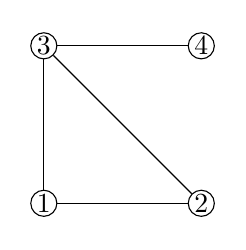
\begin{tikzpicture}
		\tikzset{tinoeud/.style={draw, circle, minimum height=0.1cm}}
		\node[tinoeud] (U) at (0,0) {};
		\node[tinoeud] (V) at (2,0) {};
		\node[tinoeud] (W) at (0,2) {};
		\node[tinoeud] (T) at (2,2) {};

    \draw (U) -- (V);
    \draw (V) -- (W);
    \draw (W) -- (U);
    \draw (W) -- (T);

    \draw (U) node {$1$};
    \draw (V) node {$2$};
    \draw (W) node {$3$};
    \draw (T) node {$4$};

		\end{tikzpicture}

		\begin{tikzpicture}
		
		\coordinate (O) at (0,0);

    \prgrid{O}{22}{22}

    \prvtline{O}{6}{22}
    \prvtline{O}{10}{22}
    \prvtline{O}{14}{22}
    \prvtline{O}{18}{22}
    
    \prvtcolumn{O}{6}{22}
    \prvtcolumn{O}{10}{22}
    \prvtcolumn{O}{14}{22}
    \prvtcolumn{O}{18}{22}
    
    \prvtdline{O}{7}{22}
    \prvtdline{O}{11}{22}
    \prvtdline{O}{15}{22}
    \prvtdline{O}{19}{22}
    
    \prvtdcolumn{O}{7}{22}
    \prvtdcolumn{O}{11}{22}
    \prvtdcolumn{O}{15}{22}
    \prvtdcolumn{O}{19}{22}
    
    \draw ($(O)+(-0.5,4)$) node {$v_1$};
    \draw ($(O)+(-0.5,6)$) node {$v_2$};
    \draw ($(O)+(-0.5,8)$) node {$v_3$};
    \draw ($(O)+(-0.5,10)$) node {$v_4$};
    
    \draw ($(O)+(4,-0.5)$) node {$v_1$};
    \draw ($(O)+(6,-0.5)$) node {$v_2$};
    \draw ($(O)+(8,-0.5)$) node {$v_3$};
    \draw ($(O)+(10,-0.5)$) node {$v_4$};

    \prbul{O}{1}{1};
    \prbul{O}{1}{2};
    \prbul{O}{1}{3};
    \prbul{O}{1}{4};
    \prbul{O}{1}{5};
    \prbul{O}{1}{6};
    
    \prbul{O}{2}{1};
    \prbul{O}{3}{1};
    \prbul{O}{4}{1};
    \prbul{O}{5}{1};
    \prbul{O}{6}{1};
 
    \prbul{O}{7}{1};
    \prbul{O}{8}{3};
    \prbul{O}{9}{3};
    \prbul{O}{9}{5};
    \prbul{O}{10}{5};
    \prbul{O}{10}{1};
 
    \prbul{O}{11}{1};
    \prbul{O}{12}{3};
    \prbul{O}{13}{3};
    \prbul{O}{13}{5};
    \prbul{O}{14}{5};
    \prbul{O}{14}{1};
 
    \prbul{O}{15}{1};
    \prbul{O}{16}{3};
    \prbul{O}{17}{3};
    \prbul{O}{17}{5};
    \prbul{O}{18}{5};
    \prbul{O}{18}{1};
 
    \prbul{O}{19}{1};
    \prbul{O}{20}{3};
    \prbul{O}{21}{3};
    \prbul{O}{21}{5};
    \prbul{O}{22}{5};
    \prbul{O}{22}{1};
		
 
    \prbul{O}{1}{7};
    \prbul{O}{3}{8};
    \prbul{O}{3}{9};
    \prbul{O}{5}{9};
    \prbul{O}{5}{10};
    \prbul{O}{1}{10};
 
    \prbul{O}{1}{11};
    \prbul{O}{3}{12};
    \prbul{O}{3}{13};
    \prbul{O}{5}{13};
    \prbul{O}{5}{14};
    \prbul{O}{1}{14};
 
    \prbul{O}{1}{15};
    \prbul{O}{3}{16};
    \prbul{O}{3}{17};
    \prbul{O}{5}{17};
    \prbul{O}{5}{18};
    \prbul{O}{1}{18};
 
    \prbul{O}{1}{19};
    \prbul{O}{3}{20};
    \prbul{O}{3}{21};
    \prbul{O}{5}{21};
    \prbul{O}{5}{22};
    \prbul{O}{1}{22};


    \prbul{O}{7}{7};
    \prbul{O}{9}{9};

    \prbul{O}{11}{11};
    \prbul{O}{13}{13};

    \prbul{O}{15}{15};
    \prbul{O}{17}{17};

    \prbul{O}{19}{19};
    \prbul{O}{21}{21};


    \prbul{O}{7}{19};
    \prbul{O}{8}{20};

    \prbul{O}{19}{7};
    \prbul{O}{20}{8};

    \prbul{O}{11}{19};
    \prbul{O}{12}{20};

    \prbul{O}{19}{11};
    \prbul{O}{20}{12};

  
    \end{tikzpicture}

\caption{This figure illustrates, on the first part, a graph in which we search for a maximum clique and, on the second part, the matrix obtained built with the reduction.}
\label{fig:reduction:example}
\end{figure}

The initial density in this matrix is $d_0 = 11 + 6|V| + (|V| (|V|-1) - 2|E|)$. Note that, firstly, only the lines $l_i$ and columns $c_i$ for $i \in \llbracket 1;n \rrbracket$ may be contracted and, secondly, we cannot increase the density of the 1's that are not contained in the gadgets $(a_i)$. In order to add one to the density of the matrix we must choose a node $v_i$ and contract the column $c_i$ and the line $l_i$. 

If the column $c_i$ is contracted and if $(v_i, v_j) \not \in E$, the two 1's of the gadget $(\beta_{i,j})$ are moved on the same column. Similarly, if the line $l_i$ is contracted, the two 1's of the gadget $(\beta_{j,i})$ are moved on the same column. This prohibits the contraction of the line $l_j$ and thecolumn $c_j$. Consequently, in order to add $C$ to the density, we must find a clique of size $C$ in the graph and contract every line and column associated with the nodes of that clique.

Thus, there is a clique of size $K$ if and only if there is a feasible solution for $M$ of density $d_0 + K$. This concludes the proof of NP-Completeness.

  \end{proof}
